\section{Auswertung}
\label{sec:Auswertung}

\section{Verwendete Stäbe}
\label{sec:Stäbe}
\paragraph{Konvention der Bezeichnungen}
\label{sec:Konvention}
Es werden ein Stab mit rundem und ein Stab mit quadratischem Querschnitt verwendet. Alle dem runden Stab zugehörigen Werte erhalten den Index $r$, die des eckigen $q$.

\paragraph{Charakteristika der Stäbe}
Der runde Stab besitzt einen Durchmesser $d$ von $10mm$ bei einer Länge $l_{r}$ von $57.5cm$ und einer Masse $m_{r}$ von $379.2g$.
Für den eckigen Stab wurden die nötigen Daten wie folgt ermittelt:

\begin{equation*}
  a = 10mm \\
  l_{q} = 60cm \\
  m_{q} = 502.4g \\
\end{equation*}

Hierbei bezeichnet $a$ die Kantenlänge des Querschnittes. Hieraus ergeben sich die Dichten $\rho_{r} = 8396.7\frac{kg}{m^3}$ und $\rho_{q} = 8373.3\frac{kg}{m^3}$. Dies entspricht etwa der Dichte von  Messing CuZn39Pb3 von $\rho_{Messing} = 8.47\frac{g}{cm^3}$ \cite{DKI}. Es wird dementsprechend davon ausgegangen, dass es sich bei beiden Stäben um Messingstäbe handelt, welche ein Elastizitätsmodul von ca. $E_Messing = 97 \frac{kN}{mm^3}$ \cite{DKI} aufweisen sollten. Folglich wird dies von nun an als Vergleichswert verwendet. 

\subsection{Einseitige Einspannung}
\label{sec:Einseitig}

\begin{table}
  \centering
\caption{Auslenkung des runden Stabes bei einseitiger Einspannung}
\label{tab:rund}
\sisetup{round-mode = places , round-precision = 2}
\begin{tabular}{S S S S}
  \toprule
  {$\symup{x}/cm$} & {$\symup{D}_0/mm$} & {$\symup{D}_m/mm$} {$\delta \symup{D}/mm$}\\
  \midrule
  \include('../Werte/V103-Reihe1-tab.txt')
\bottomrule
\end{tabular}
\end{table}
\FloatBarrier

\begin{table}
  \centering
\caption{Auslenkung des eckigen Stabes bei einseitiger Einspannung}
\label{tab:eckig}
\sisetup{round-mode = places , round-precision = 2}
\begin{tabular}{S S S S}
  \toprule
  {$\symup{x}/cm$} & {$\symup{D}_0/mm$} & {$\symup{D}_m/mm$} {$\delta \symup{D}/mm$}\\
  \midrule
  \include('../Werte/V103-Reihe3-tab.txt')
\bottomrule
\end{tabular}
\end{table}
\FloatBarrier

Die bei einseitiger Einspannung des runden Stabes ermittelten Werte lassen sich der Tabelle \ref{tab:rund} entnehmen, wobei $\symup{D}_0$ die Auslenkungen im unbelasteten Fall darstellt, $\symup{D}_m$ die im belasteten und $\symup{x}$ die Position entlang des Stabes (Einspannung bei $\symup{x}=0$). Hierbei wird eine Belastung von $m_1 = 379.2g$ gewählt. Ihre graphische Darstellung lässt sich Abb. \ref{fig:Reihe1} entnehmen.
Für den eckigen Stab (Tabelle \ref{tab:eckig}) ist $m_2 = 767.5g$. Seine Auslenkung wird in Abb. \ref{fig:Reihe2} veranschaulicht.

Mittels Formel \eqref{eqn:I} ergeben sich sich die Flächenträgheitsmomente zu

\begin{equation}
    \symup{I}_{r} = \int_{0}^{\pi (d/2)^2} r^2 \dif{\pi r^2} = \pi^2 \left( d/2 \right)^4 = 6.17e-9 m^4
\end{equation}
 und
\begin{equation}
  \symup{I}_{q} = \int_{0}^{a^2} y^2 \dif{(2y)^2} =
\end{equation}

Aus \ref{eqn:D1} ergibt sich somit

\begin{equation}
  \symup{E}_{r} = \frac{\symup{F}}{2\symup{DI}_{r}} \left( \symup{Lx}^2 - \frac{\symup{x}^3}{3} \right) =
\end{equation}

\begin{figure}
  \centering
  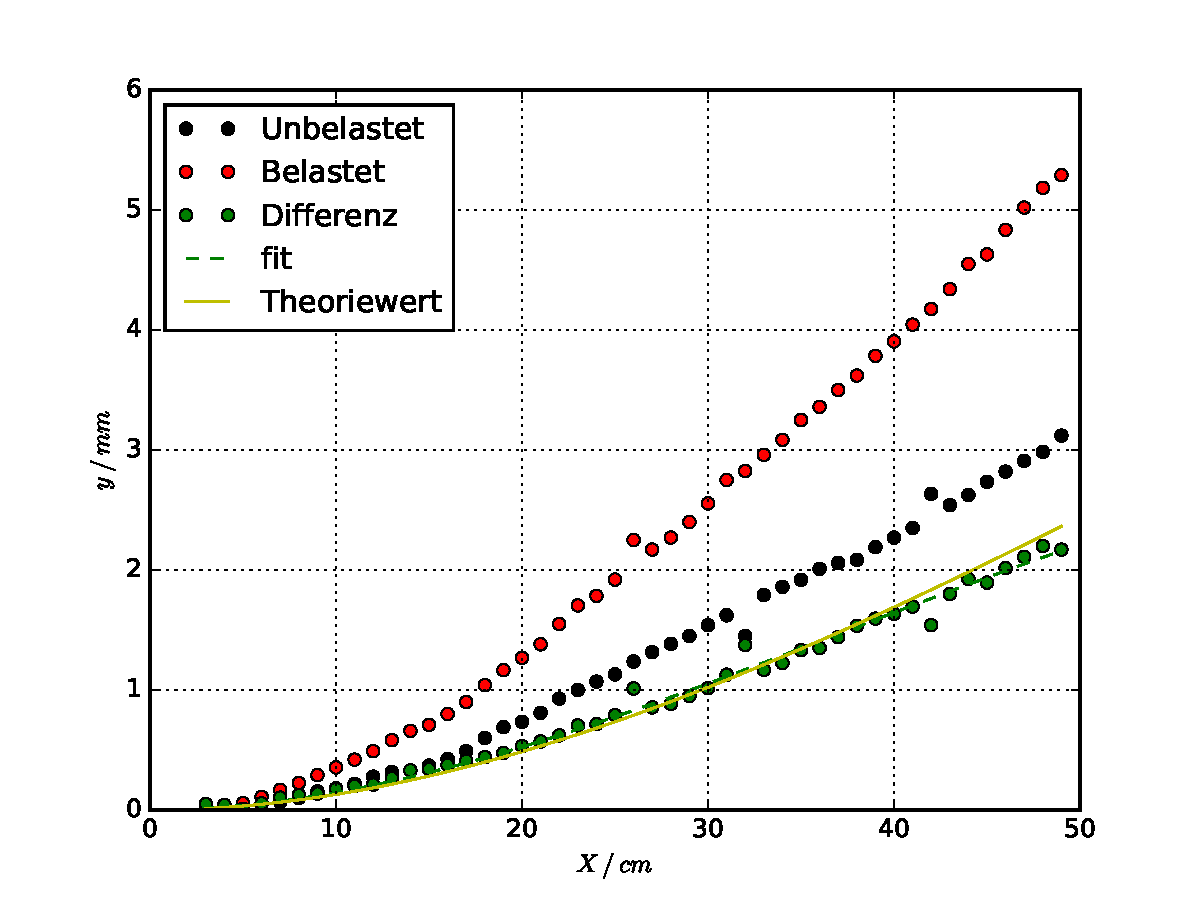
\includegraphics{/Plots/Reihe1.pdf}
  \caption{Reihe1}
  \label{fig:Reihe1}
\end{figure}

\begin{figure}
  \centering
  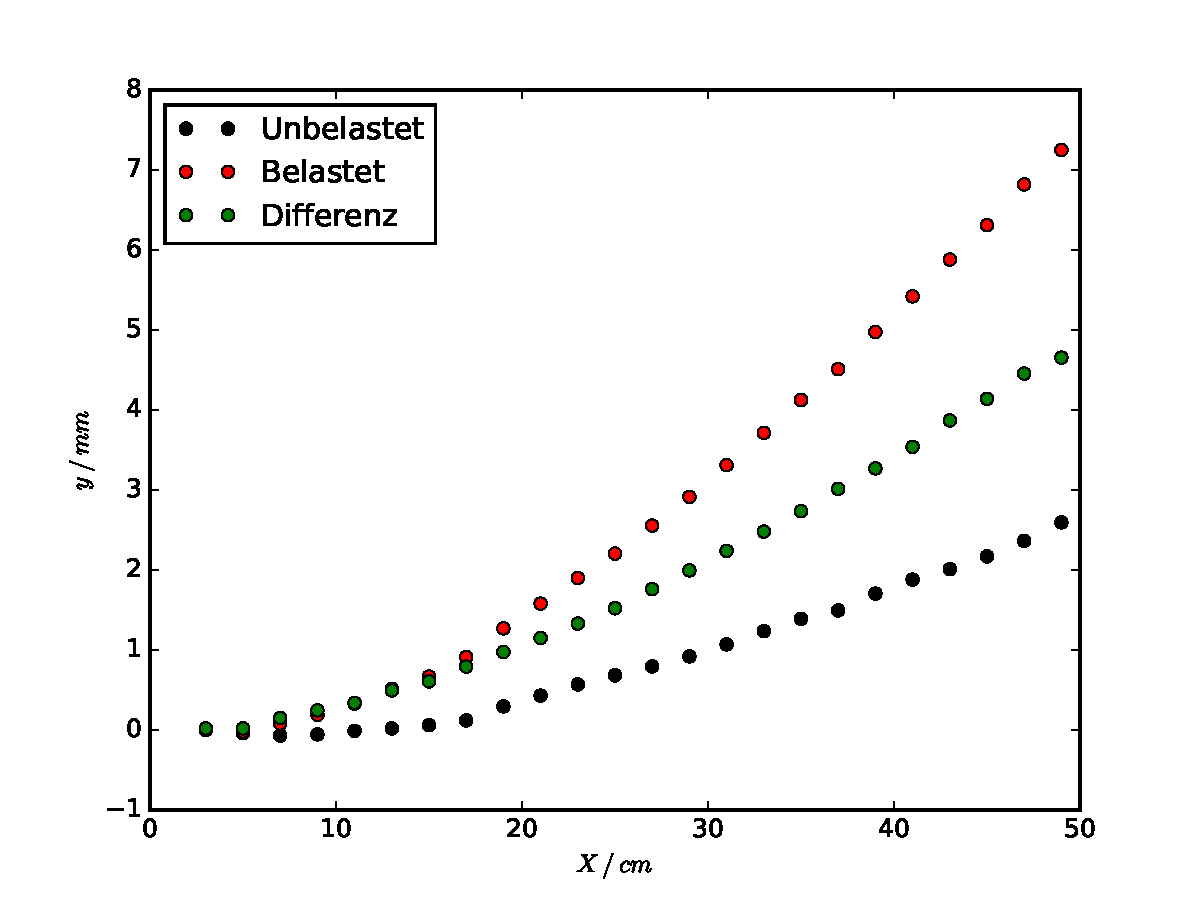
\includegraphics{/Plots/Reihe2.pdf}
  \caption{Reihe2}
  \label{fig:Reihe2}
\end{figure}
\FloatBarrier

\subsection{Beidseitige Auflage}
\label{sec:Beidseitig}

\begin{table}
  \centering
\caption{Auslenkung des runden Stabes bei beidseitiger Auflage}
\label{tab:rundBeidseitig}
\sisetup{round-mode = places , round-precision = 2}
\begin{tabular}{S S S S}
  \toprule
  {$x/cm$} & {$D_0/mm$} & {$D_m'/mm$} {$\delta D/mm$}\\
  \midrule
  \include('../Werte/V103-Reihe2-tab.txt')
\bottomrule
\end{tabular}
\end{table}
\FloatBarrier

In diesem letzten Verfahren wird der runde Stab mit $m_{3}=4722.5g$ mittig belastet. Durch die Aufhängung des Gewichtes ist es nicht möglich, zwischen $x = 25cm$ und $x = 30cm$ die Auslenkung zu bestimmen (siehe Tabelle \ref{tab:rundBeidseitig}, bzw. Abb. \ref{fig:Reihe3})

\begin{figure}
  \centering
  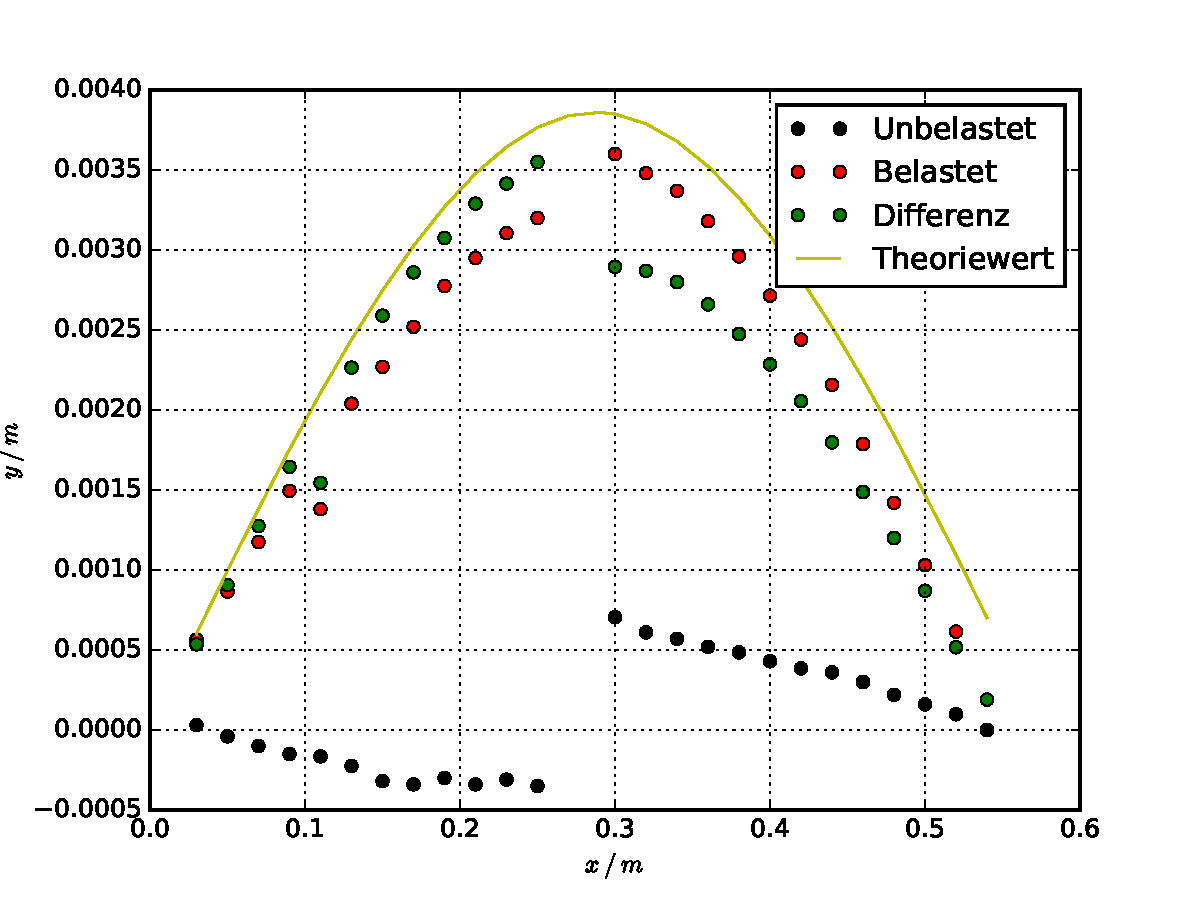
\includegraphics{/Plots/Reihe3.pdf}
  \caption{Reihe3}
  \label{fig:Reihe3}
\end{figure}
